\subsection{Getting Started with the FFW}
\label{sect:QuickStart:gettingStarted}

\noindent This Subsection will tell you how to execute an existing script for a problem and how to manipulate it.\medskip

\noindent In the following we will consider the problem to calculate the solution of an elliptic PDE, i.e.
\begin{align*}
- \ddiv (\kappa \,\grad u) + \lambda \,\grad u + \mu \, u &= f &&\text{in } \Omega,\\
u &= u_D &&\text{on } \Gamma,\\
\frac{\partial u}{\partial n} &= g &&\text{on } \partial\Omega \setminus \Gamma.
\end{align*}
To keep it simple, we set $\kappa = I$, $\lambda = 0$, $\mu = 0$, $f \equiv 1$, $u_D \equiv 0$ and $g \equiv 0$, on a L-shaped domain $\Omega$ with Dirichlet boundary only (Neumann boundary $\partial\Omega \setminus \Gamma = \emptyset$).\medskip

\noindent First, take a look at the script in Figure~\ref{sect:Quickstart.fig.code:gettingStarted}, which is located in the root folder of the \FFW\!.

\begin{figure}[ht!]
\inputcoden{../gettingStarted.m}
\caption{Content of \code{gettingStarted.m}}\label{sect:Quickstart.fig.code:gettingStarted}
\end{figure}

\medskip
\noindent To start a script, set MATLAB's current directory to the root of the \FFW and execute it. Any script you want to use with the \FFW has to be located in the root folder of the \FFW\!.\medskip

\noindent 
\begin{enumerate}[{\hspace{15mm}}]
\item[Line 3:] The name of a file that describes the problem is defined. This file is located at \path{.\problems\elliptic\}. The content of this file is shown in Figure~\ref{sect:Quickstart.fig.code:problem}. For more details on the geometry refer to Section~\ref{sect:DataStructures}. For more details on the problem definition see also Subsection~\ref{sect:QuickStart:ProblemDefinition}.
\item[Line 4:] The type of finite element method is chosen. This can possibly also be \code{'CR'}.
\item[Line 5:] This is the indicator when to stop the refinement, i.e., the calculations. For more details refer to Section~\ref{sect:MeshGeneration}.
\item[Line 6:] The mark algorithm is chosen. The argument can also be \code{'maximum'} or \code{'uniform'}. For more details refer to Section~\ref{sect:MeshGeneration}.
\item[Line 8:] The \FFW is initialized with the above arguments, i.e., the structure \code{p} is created. The last argument describes what problem type is to be computed. This argument can possibly also be \code{'elasticity'}. See also Section~\ref{sect:ImplementedProblems}.
\item[Line 9:] The actual calculations are started. See also Section~\ref{sect:FlowChart} for details.
\item[Line 12:] The solution is plotted with the standard parameters. More details about the \code{show} function as well as its parameters can be found in Section~\ref{sect:GraphicalOutput}.
\item[Line 15:] The estimated error is plotted with the standard parameters.
\end{enumerate}
\bigskip

\noindent For the results, i.e. the solution and the estimated error, of the \code{gettingStarted.m} script, see Figure~\ref{sect:Quickstart.fig.plots.gettingStarted}.

\begin{figure}[ht!]
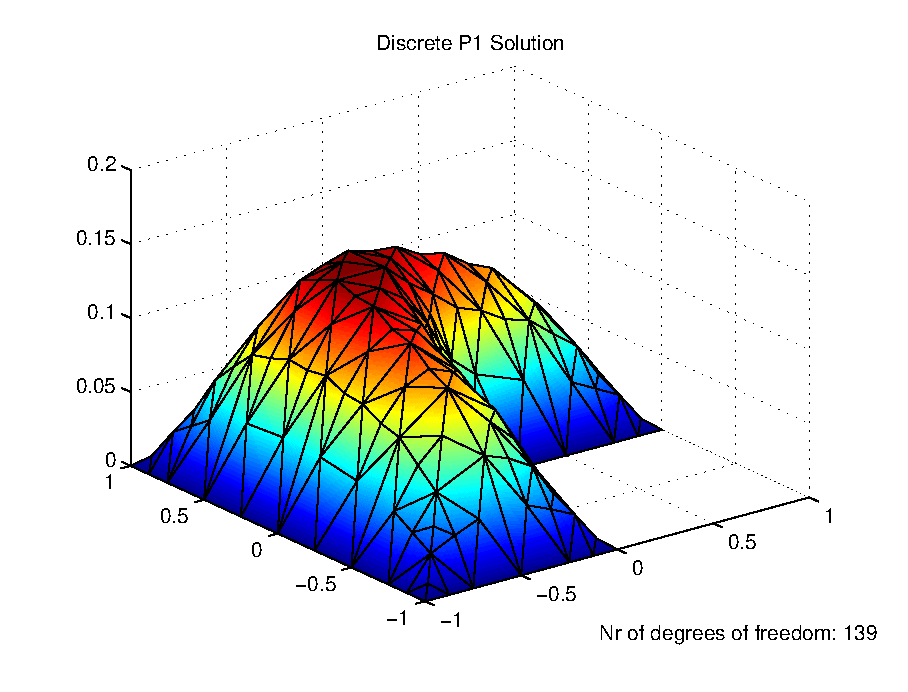
\includegraphics[width= 0.49\textwidth]{images/sect_QuickStart_LShapeU1}
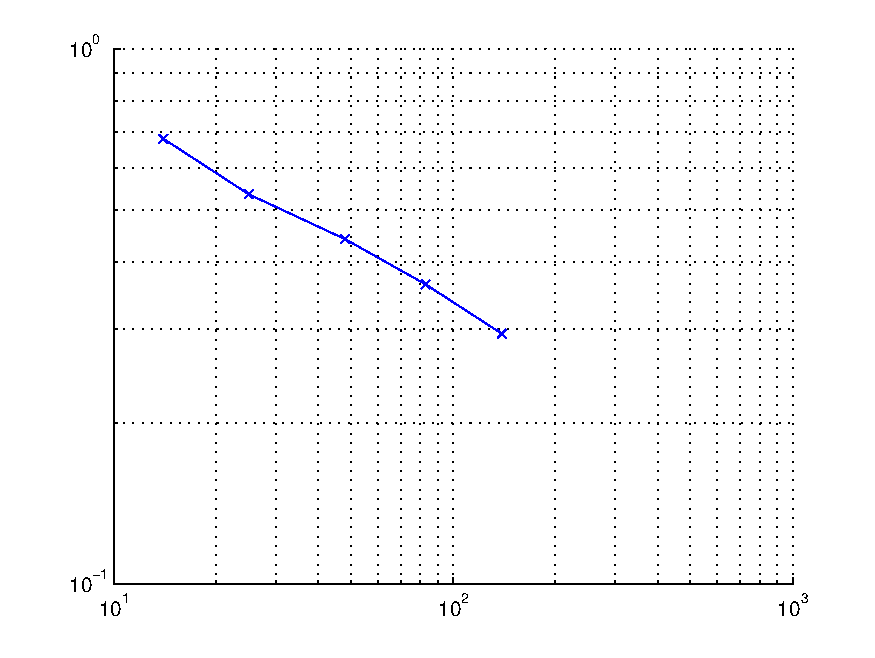
\includegraphics[width= 0.49\textwidth]{images/sect_QuickStart_LShapeE1}\\
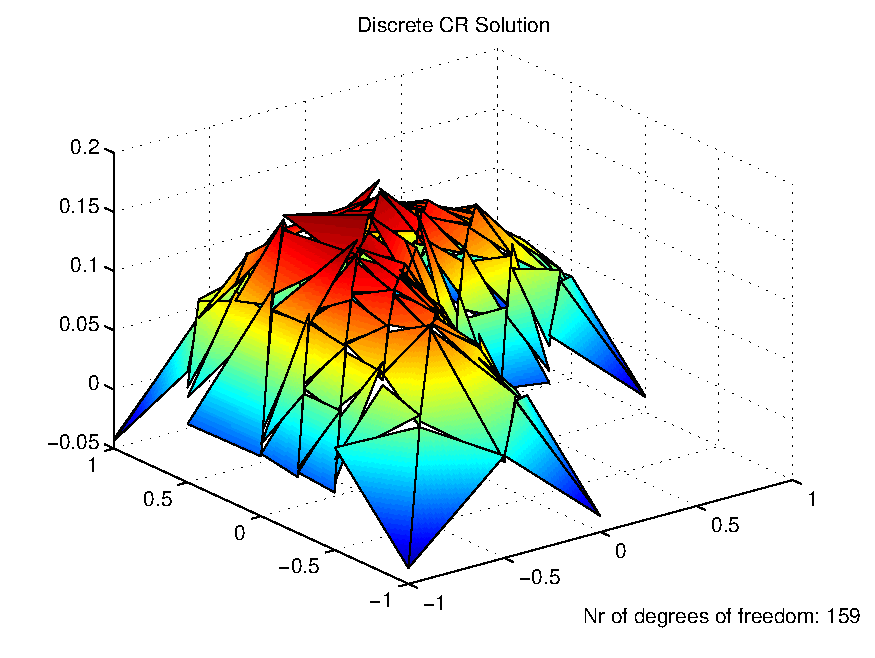
\includegraphics[width= 0.49\textwidth]{images/sect_QuickStart_LShapeU2}
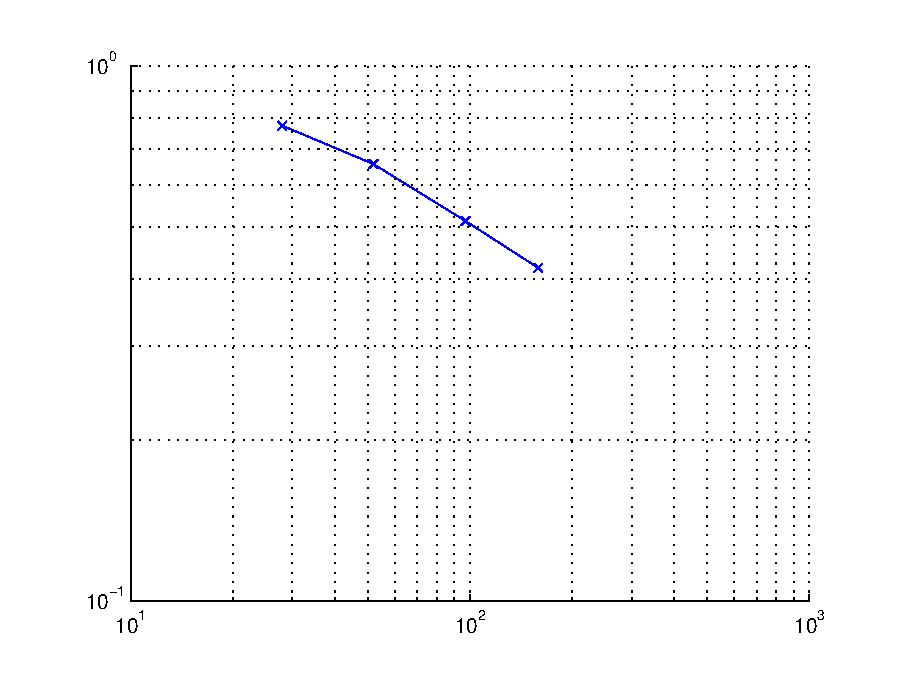
\includegraphics[width= 0.49\textwidth]{images/sect_QuickStart_LShapeE2}
\caption{Plots obtained from the \code{gettingStarted.m} script for \code{pdeSolver = 'P1'} on top and \code{pdeSolver = 'CR'} below.}\label{sect:Quickstart.fig.plots.gettingStarted}
\end{figure}

\bigskip
\noindent To make it more convenient to work with the \FFW, there are `startscripts' with almost all available PDE solvers, already implemented problems and different draw routines, for elliptic and elasticity problems respectively. Those scripts can be found in the root folder (\code{startElasticity.m} and \code{startElliptic.m}).\bigskip

\noindent For a more complex example, see the script in Figure~\ref{sect:Quickstart.fig.code:advancedExample} or the script file \path{advancedExample.m} in the root directory of the \FFW\!. This scripts implements the so called `waterfall' example on a square domain.

\begin{figure}[ht!]
\inputcode{../advancedExample.m}
\caption{Content of \code{advancedExample.m}}\label{sect:Quickstart.fig.code:advancedExample}
\end{figure}
\clearpage